\begin{secao}{Tudo Que Vai Volta (até bixo)}
%TODO ARRUMAR TUDO! Ver as linhas, colocar mapa de circular, etc etc.
\begin{subsecao}{Ônibus}

Se você é um bixo que não tem como ir nem como voltar, temos algumas dicas:

\begin{enumerate}
  \item Trabalhe muito para comprar um carro,
  trabalhe mais para pagar a gasolina,
  venha para a USP de carro e, obrigatoriamente, dê carona a um VETERANO;

  \item Peça a uma pessoa amiga para trazê-lo e buscá-lo durante seus
  longos anos de IME;

  \item Conheça alguém que, por sorte, mora perto da sua casa, estuda na USP,
  tenha o mesmo horário que você, seja legal e tenha carro. Traduzindo, s-o-n-h-e;

  \item Estique o dedão e espere, espere, espere, espere... a boa vontade
  de alguém para te dar carona;

  \item Mude-se para uma casa perto da USP;

  \item Desista do curso e diga: ``Eu não queria mesmo!!'';
\end{enumerate}

OK, você decidiu ser um bixo normal e vai pegar ônibus! Mas você não sabe nem 
dar sinal pra ele parar né? Sem problemas, vamos tentar te ajudar!

Se você vai usar ônibus para ir ou voltar da USP, você precisa conhecer
basicamente dois pontos de ônibus: o ponto da FAU e o ponto da
FEA. Ambos ficam na Av. Prof. Luciano Gualberto (que a partir de agora será
chamada de Rua dos Bancos, para todo e todo o sempre).

Para tentar facilitar:
\begin{itemize}
	\item Av. Prof. Luciano Gualberto = Rua dos Bancos;
	\item Av. Prof. Lineu Prestes = Rua do HU;
	\item Av. Prof. Mello Moraes = Rua da Raia.
\end{itemize}

O mais provável é que você chegue na USP por um desses
pontos e vá embora pelo outro. 

Esses dois pontos ficam em lados opostos da Rua dos Bancos, um de frente para o
outro, basta atravessar a rua. 

Aqui está a lista de ônibus que passam em cada um dos pontos. Para mais detalhes
sobre cada linha, você pode usar o site da SPTrans ou o Google Maps.

{\bf Linhas municipais:}

{\bf Ponto da FAU}

(Esses te levam pra fora da USP)
\begin{center}
	\begin{tabular}{|c|c|c|}
      \hline
	  Letreiro & Cor & Interligações (em ordem)\\
	  \hline
	  177H-10 - Metrô Santana & Azul & Metrô: L4, L2, L3 e L1\\
	  7181-10 - Term. Princ. Isabel & Laranja & CPTM: L9\\
	  7411-10 - Praça da Sé & Laranja & Metrô: L4, L2, L3 e L1\\
	  7725-10 - Rio Pequeno & Laranja & - \\
	  8022-10 - Metrô Butantã* & Laranja & CIRCULAR USP\\
      \hline
	\end{tabular}
\end{center}

Esses dois ônibus passam no ponto, mas estão CHEGANDO na USP, portanto não seja
ridículo dando sinal para eles pararem e muito menos pegue um desses ônibus
nesse ponto.

\begin{center}
	\begin{tabular}{|c|c|}
	  \hline
	  Letreiro & Cor\\
	  \hline
	  701U-10 - Butantã-USP & Azul\\
	  702U-10 - Butantã-USP & Laranja\\
	  \hline
	\end{tabular}
\end{center}

{\bf Ponto da FEA}

(Esses te levam pra fora da USP)
\begin{center}
	\begin{tabular}{|c|c|c|}
      \hline
	  Letreiro & Cor & Interligações (em ordem)\\
	  \hline
	  701U-10 - Metrô Santana & Azul & Metrô: L4, L2, L3 e L1\\
	  702U-10 - Term. Pq. D.Pedro II & Laranja & Metrô: L4, L2 e L3\\
	  7725-10 - Terminal Lapa & Laranja & CPTM: L8\\
	  8012-10 - Metrô Butantã* & Laranja & CIRCULAR USP\\
      \hline
	\end{tabular}
\end{center}

Novamente, esses três ônibus passam no ponto, mas estão CHEGANDO na USP!
\begin{center}
	\begin{tabular}{|c|c|}
	  \hline
	  Letreiro & Cor\\
	  \hline
	  177H-10 - Butantã-USP & Azul\\
	  7181-10 - Cidade Universitária & Laranja\\
	  7411-10 - Cidade Universitária & Laranja\\
	  \hline
	\end{tabular}
\end{center}

As linhas marcadas com um * são as linhas circulares da SPTrans. Segue abaixo suas descrições!

{\bf Circulares:}

Também conhecido como ``circulenda'' ou ``secular'' (aos sábados, ``milenar'', e aos domingos, ``anos-luz''), é o meio de transporte mais barato dentro da USP. Foi criado para os USPianos se locomoverem dentro do Campus, mas em muitas vezes é melhor andar do que ficar esperando. Existem 2 itinerários distintos, com trajetos aproximadamente reversos. Fique atento para não dar uma de bixo burro (duh!) e se perder, hein? 

Há controvérsias incontáveis, mas há circulares aos fins-de-semana, bixo dedicado. Surge uma terceira linha chamada “Museus”, e fica a cargo do leitor adivinhar por onde ela passa. De qualquer forma, é um itinerário alterado com notável frequência... No último modelo conhecido, os pontos mais próximos para vir para o IME, seriam: para quem vem do P3, o Acesso Vila Indiana, e então se deve descer TODA a Rua do Estupro por vezes chamada de Rua do Matão, e para quem vem do P1, o ponto da FEA. Vale comentar que, aos sábados, esses ônibus passam a cada uma hora e meia, e, aos domingos, existe uma média de 2 circulares passando num ponto, com margem de erro igual a 3. 

Em 2012 foram implantadas as linhas 8012/10 e 8022/10 - Metro Butantã/Cidade Universitária, que funcionam como circulares USP, e nós alunos não pagamos, pois elas aceitam o bilhete USP (BUSP - Retire logo o seu!!).

Como sabemos que alguns bixos ainda tem dificuldade com a leitura, colocamos o
 mapa das duas linhas no fim da seção!


{\bf Linhas intermunicipais:}

Agora, se você mora mais longe ainda (outra cidade, outro estado, outro país...) e não quer ou não pode se mudar para São Paulo, existem algumas linhas de ônibus fretados para cidades mais próximas (ou não). Se por acaso a sua cidade não está aí, procure se informar a respeito, pois não significa necessariamente que não haja ônibus da USP para lá. Aí estão elas:

\begin{itemize}
  \item {\bf Empresa Urubupungá.}\\
    Tel: 3658-7777
    Site: {\tt www.urubupunga.com.br}\\
    280BI1- São Bernardo do Campo (Centro)\\
    Cor: Cinza\\
    Onde pegar para sair da USP: ponto da FAU\\
    Av Magalhães de Castro, Av Marginal Pinheiros (Shopping Eldorado), Av Dos
    Bandeirantes, Av Eng. Luiz Carlos Berrini, Av Roque Petroni Jr. (Shopping
    Morumbi), Av Prof Vicente Rão, Av Cupecê (Diadema), Av Fábio Eduardo Ramos
    Esquivel (Diadema), Av Piraporinha (Diadema), Av Lucas Nogueira Garcez
    (Diadema), Av Urubupungá.

  \item {\bf Fretados Jundiaí - USP}\\
    Viação MIMO\\
    Tel: 4522-7788\\
    {\tt www.viacaomimo.com.br}\\
    Principais horários:\\
    Ida: 6h20; 7h20; 12h50; 18h00 (na Rodoviaria de Jundiaí)\\
    Volta: 11h50; 17h20; 23h00 (No ponto da FEA)

  \item {\bf São José dos Campos}\\
    Redenção\\
    tel: (12) 3931-3047\\
    {\tt www.redencaoturismo.com.br}\\
    Ida: 06h15 (na gruta em S. José)\\
    Volta:17h40 (no ponto da p2)

  \item {\bf Bragança}\\
    N.S. Fátima\\
    {\tt www.saexbra.com.br}\\
    Tel: 4032-4723 e 7344-2007\\
    Ida: 05h50 (Lgo do Tabão/Habbibs)\\
    Volta:17h00 (Av prof almeida Prado)

  \item {\bf Campinas}\\
    Sta. Cruz\\
    Tel:3868-5995\\
    {\tt www.gruposantacruz.com.br}

  \item {\bf Santos}\\
    Náutica Turismo\\
    Tel: (13) 9112-8860

  \item {\bf Santos / S. Vicente}\\
    Transul\\
    Tel: 6954-4466

  \item {\bf ABC}\\
    Dinâmica ABC-USP\\
    4352-0565 / 4109-0172

  \item {\bf Sorocaba}\\
    Fretado Diurno\\
    (15) 9715-1676 (Márcio)

  \item {\bf Van (diurno e noturno)}\\
    RR transportes\\
    6919-3345 / 7144-3934\\
    4474-1222 \\

\end{itemize}

\end{subsecao}

\begin{figure}[H]
    \centering
    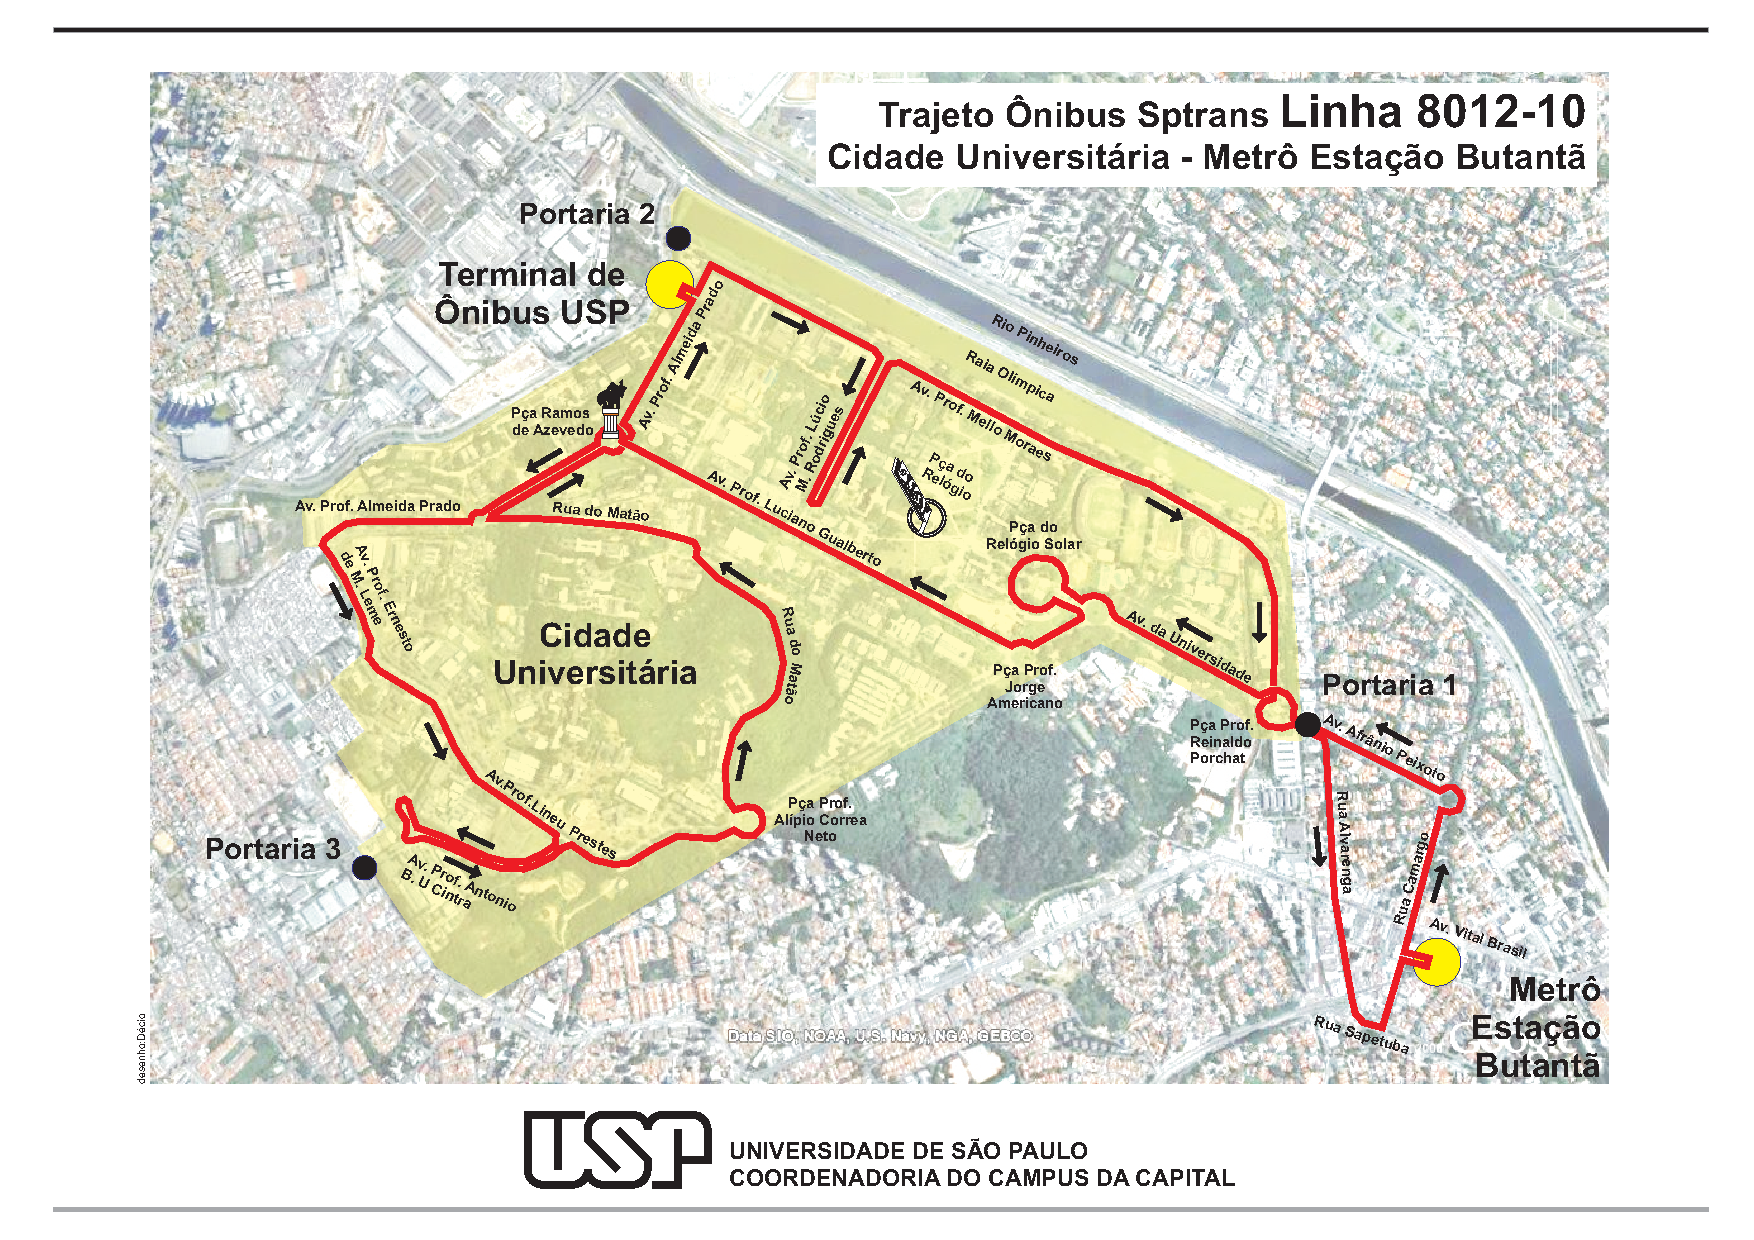
\includegraphics[height=\textwidth, angle=90]{img/8012-10.pdf}
\end{figure}

\begin{figure}[H]
  \begin{center}
    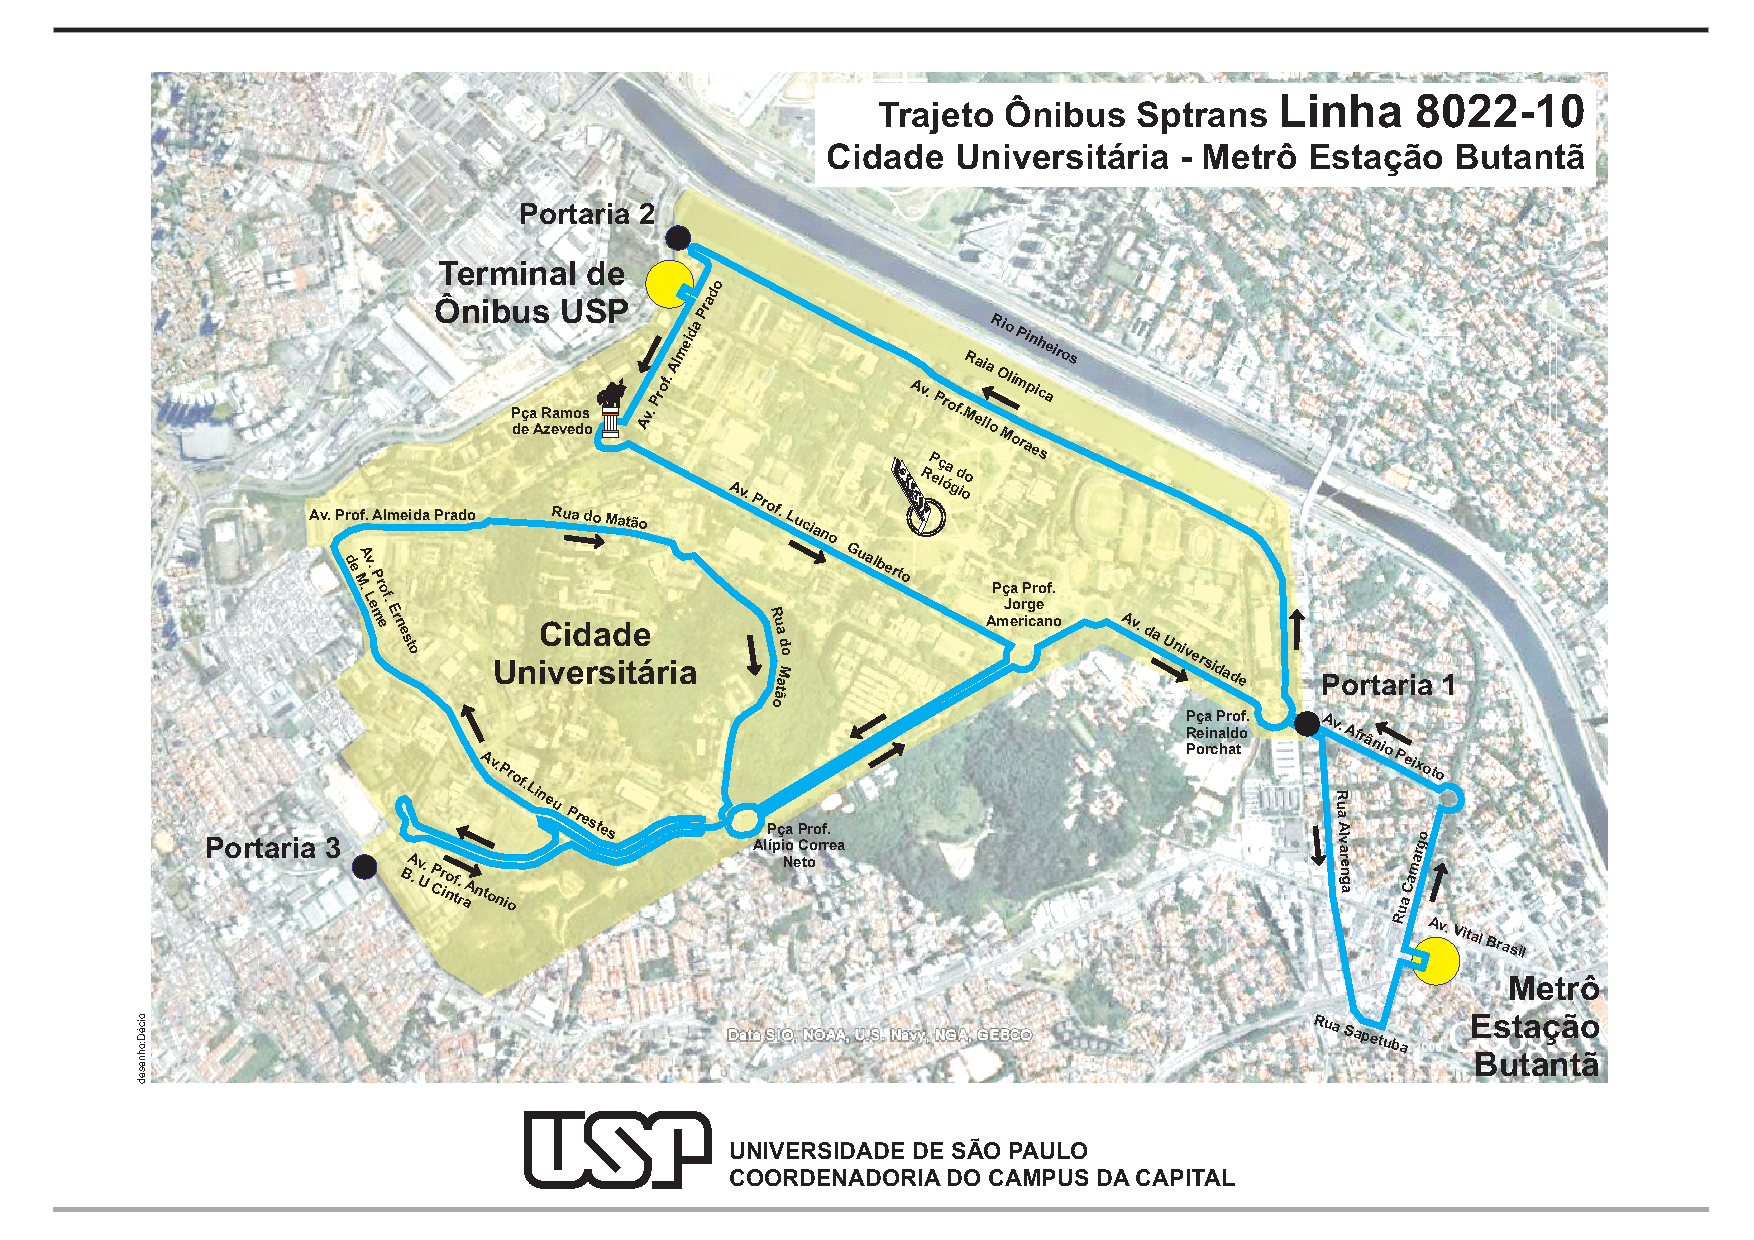
\includegraphics[height=\textwidth, angle=90]{img/8022-10.pdf}
  \end{center}
\end{figure}


\begin{subsecao}{Veículos no Campus}
Saiba por onde entrar na USP. Lembre-se de ter sempre a sua carteirinha USP ou
seu comprovante de matrícula com RG em mãos. 
\begin{itemize}
  \item {\bf Portaria 1 (P1):} R. Afrânio Peixoto. Funciona 24h por dia todos os
    dias, mas a entrada é controlada de segunda à sexta das 20h às 05h, aos sábados
    após as 14h e domingo o dia inteiro. É por onde entram os ônibus municipais. 
    
  \item {\bf Portaria 2 (P2):} Av. Escola Politécnica. Funciona das 5h30 às 20h
    de segunda a sexta. Entrada controlada de seg a sex das 20h às 24h. Fechada
    aos sábados, domingos e feriados. Única entrada para caminhões. 
    
  \item {\bf Portaria 3 (P3):} Av. Corifeu de Azevedo Marques. Tem o mesmo horário
    de funcionamento da P2.

  \item {\bf Portaria 1/2:} R. Eng. Teixeira Soares. Funciona de segunda a sexta das 5h30 às 20h. 
    
  \item {\bf Portarias de pedestre (Mercadinho, São Remo, HU, FEPASA e
      Vila Indiana):} Funcionam de 2ª a 6ª, das 05 às 23 hs.

\end{itemize}

Aos fins de semana, ficam abertas apenas as portarias 1 e 3 (esta, fecha mais cedo). É preciso se identificar.

Os ônibus entram no sábado até as 14h e não entram no domingo. Se você vem de carro, saiba que a universidade dispões de bolsões de estacionamento
gratuito em torno das Unidades.

\end{subsecao}

\begin{subsecao}{Pontos de táxi}
Existem alguns pontos de táxi espalhados pela Cidade Universitária. Eis suas
localidades:

\begin{itemize}
\item Ponto da FEA / ECA (atrás do Banespa)\\
Fone: 3091-4488

\item Ponto da Reitoria\\
Fone: 3091-3556

\item Ponto do Hospital Universitário\\
Fone: 3091-3536
\end{itemize}
\end{subsecao}


\end{secao}
